%%%%%%%%%%%%%%%%%%%%%%%%%%%%%%%%%%%%%%%%%%%%%%%%%%%%%%%%%%%%%%%
%% OXFORD THESIS TEMPLATE

% Use this template to produce a standard thesis that meets the Oxford University requirements for DPhil submission
%
% Originally by Keith A. Gillow (gillow@maths.ox.ac.uk), 1997
% Modified by Sam Evans (sam@samuelevansresearch.org), 2007
% Modified by John McManigle (john@oxfordechoes.com), 2015
%
% This version Copyright (c) 2015-2023 John McManigle

% This file is commented extensively, so read through it to see how to use the various options.  Remember
% that in LaTeX, any line starting with a % is NOT executed.  Several places below, you have a choice of which line to use
% out of multiple options (eg draft vs final, for PDF vs for binding, etc.)  When you pick one, add a % to the beginning of
% the lines you don't want.


%%%%% CHOOSE PAGE LAYOUT
% The most common choices should be below.  You can also do other things, like replacing "a4paper" with "letterpaper", etc.

% This one will format for two-sided binding (ie left and right pages have mirror margins; blank pages inserted where needed):
% \documentclass[a4paper,twoside]{ociamthesis}
% This one will format for one-sided binding (ie left margin > right margin; no extra blank pages):
%\documentclass[a4paper]{ociamthesis}
% This one will format for PDF output (ie equal margins, no extra blank pages):
\documentclass[a4paper,nobind]{ociamthesis} 


%%%%% DATE FORMAT SETUP
\usepackage{datetime}
\newdateformat{specialdate}{\THEDAY\ \monthname[\THEMONTH]\ \THEYEAR}


%%%%% SELECT YOUR DRAFT OPTIONS
% Three options going on here; use in any combination.  But remember to turn the first two off before
% generating a PDF to send to the printer!

% This adds a "DRAFT" footer to every normal page.  (The first page of each chapter is not a "normal" page.)
\fancyfoot[C]{\emph{DRAFT Printed on \specialdate\today}}  

% This highlights (in blue) corrections marked with (for words) \mccorrect{blah} or (for whole
% paragraphs) \begin{mccorrection} . . . \end{mccorrection}.  This can be useful for sending a PDF of
% your corrected thesis to your examiners for review.  Turn it off, and the blue disappears.
\correctionstrue


%%%%% BIBLIOGRAPHY SETUP
% Note that your bibliography will require some tweaking depending on your department, preferred format, etc.
% The options included below are just very basic "sciencey" and "humanitiesey" options to get started.
% If you've not used LaTeX before, I recommend reading a little about biblatex/biber and getting started with it.
% If you're already a LaTeX pro and are used to natbib or something, modify as necessary.
% Either way, you'll have to choose and configure an appropriate bibliography format...

% The science-type option: numerical in-text citation with references in order of appearance.
% \usepackage[style=numeric-comp, sorting=none, backend=biber, doi=false, isbn=false]{biblatex}
% \newcommand*{\bibtitle}{References}

% The humanities-type option: author-year in-text citation with an alphabetical works cited.
\usepackage[style=apa, backend=biber]{biblatex}
\newcommand*{\bibtitle}{Bibliography}

% This makes the bibliography left-aligned (not 'justified') and slightly smaller font.
\renewcommand*{\bibfont}{\raggedright\small}

% Change this to the name of your .bib file (usually exported from a citation manager like Zotero or EndNote).
\addbibresource{references.bib}


% Uncomment this if you want equation numbers per section (2.3.12), instead of per chapter (2.18):
%\numberwithin{equation}{subsection}



%%%%% THESIS / TITLE PAGE INFORMATION
% Everybody needs to complete the following:
\title{Suitably impressive thesis title}
% \author{Your Name}
% \college{Your College}

% Master's candidates who require the alternate title page (with candidate number and word count)
% must also un-comment and complete the following three lines:
\masterssubmissiontrue
\candidateno{1069672}
\wordcount{28,815}

% Uncomment the following line if your degree also includes exams (eg most masters):
\renewcommand{\submittedtext}{Submitted in partial completion of the}
% Your full degree name.
\degree{Master of Philosophy in Sociology and Demography}
% Term and year of submission, or date if your board requires (eg most masters)
\degreedate{\specialdate\today}


%%%%% YOUR OWN PERSONAL MACROS
% This is a good place to dump your own LaTeX macros as they come up.

% To make text superscripts shortcuts
	\renewcommand{\th}{\textsuperscript{th}} % ex: I won 4\th place
	\newcommand{\nd}{\textsuperscript{nd}}
	\renewcommand{\st}{\textsuperscript{st}}
	\newcommand{\rd}{\textsuperscript{rd}}

%%%%% THE ACTUAL DOCUMENT STARTS HERE
\begin{document}



%%%%% CHOOSE YOUR LINE SPACING HERE
% This is the official option.  Use it for your submission copy and library copy:
\setlength{\textbaselineskip}{22pt plus2pt}
% This is closer spacing (about 1.5-spaced) that you might prefer for your personal copies:
%\setlength{\textbaselineskip}{18pt plus2pt minus1pt}

% You can set the spacing here for the roman-numbered pages (acknowledgements, table of contents, etc.)
\setlength{\frontmatterbaselineskip}{17pt plus1pt minus1pt}

% Leave this line alone; it gets things started for the real document.
\setlength{\baselineskip}{\textbaselineskip}


%%%%% CHOOSE YOUR SECTION NUMBERING DEPTH HERE
% You have two choices.  First, how far down are sections numbered?  (Below that, they're named but
% don't get numbers.)  Second, what level of section appears in the table of contents?  These don't have
% to match: you can have numbered sections that don't show up in the ToC, or unnumbered sections that
% do.  Throughout, 0 = chapter; 1 = section; 2 = subsection; 3 = subsubsection, 4 = paragraph...

% The level that gets a number:
\setcounter{secnumdepth}{4}
% The level that shows up in the ToC:
\setcounter{tocdepth}{4}


%%%%% ABSTRACT SEPARATE
% This is used to create the separate, one-page abstract that you are required to hand into the Exam
% Schools.  You can comment it out to generate a PDF for printing or whatnot.
% \begin{abstractseparate}
% 	\begin{itemize}
    \item \textbf{Background}: As digital technologies increasingly permeate all aspects of society, particularly healthcare, understanding the role of digital literacy in shaping health outcomes among older adults becomes crucial. This thesis investigates the impact of digital literacy on health outcomes and assesses whether heightened digitalisation has exacerbated health disparities between older adults with varying levels of digital literacy.
    \item \textbf{Methodology}: Utilising data from the English Longitudinal Study of Ageing, this study employs quantitative analysis techniques to explore the relationship between digital literacy levels and various health outcomes among older adults. It specifically examines the causal effect of digital literacy on health through Inverse Probability of Treatment Weighting and investigates whether increased digitalisation exacerbates health inequalities using a Matching Difference-in-Difference approach.
    \item \textbf{Results}: The findings suggest that higher levels of digital literacy lead to better health outcomes, indicating that proficiency in digital tools is integral to managing health effectively in a digital age. Additionally, the study reveals that increased digitalisation tends to widen health disparities among those with different levels of digital literacy, highlighting a growing divide in health equity related to digital skills.
    \item \textbf{Conclusion}: This thesis underscores digital literacy as a significant determinant of health among older adults, providing evidence for policymakers to foster digital education and skill development to bridge health disparities. By enhancing digital literacy, health equity can be improved, making the benefits of digital healthcare more universally accessible.
\end{itemize} % Create an abstract.tex file in the 'text' folder for your abstract.
% \end{abstractseparate}


% JEM: Pages are roman numbered from here, though page numbers are invisible until ToC.  This is in
% keeping with most typesetting conventions.
\begin{romanpages}

% JEM: By default, this template uses the traditional Oxford "Belt Crest". Un-comment the following
% line to use the newer, "Blue Square" logo:
% \renewcommand{\crest}{{\includegraphics[width=4.2cm, height=4.2cm]{figures/newlogo.pdf}}}

% Title page is created here
\maketitle

%%%%% DEDICATION -- If you'd like one, un-comment the following.
%\begin{dedication}
%This thesis is dedicated to\\
%someone\\
%for some special reason\\
%\end{dedication}

%%%%% ACKNOWLEDGEMENTS -- Nothing to do here except comment out if you don't want it.
% \begin{acknowledgements}
%  	\subsection*{Personal}

This is where you thank your advisor, colleagues, and family and friends.

Lorem ipsum dolor sit amet, consectetur adipiscing elit. Vestibulum feugiat et est at accumsan. Praesent sed elit mattis, congue mi sed, porta ipsum. In non ullamcorper lacus. Quisque volutpat tempus ligula ac ultricies. Nam sed erat feugiat, elementum dolor sed, elementum neque. Aliquam eu iaculis est, a sollicitudin augue. Cras id lorem vel purus posuere tempor. Proin tincidunt, sapien non dictum aliquam, ex odio ornare mauris, ultrices viverra nisi magna in lacus. Fusce aliquet molestie massa, ut fringilla purus rutrum consectetur. Nam non nunc tincidunt, rutrum dui sit amet, ornare nunc. Donec cursus tortor vel odio molestie dignissim. Vivamus id mi erat. Duis porttitor diam tempor rutrum porttitor. Lorem ipsum dolor sit amet, consectetur adipiscing elit. Sed condimentum venenatis consectetur. Lorem ipsum dolor sit amet, consectetur adipiscing elit.

Aenean sit amet lectus nec tellus viverra ultrices vitae commodo nunc. Mauris at maximus arcu. Aliquam varius congue orci et ultrices. In non ipsum vel est scelerisque efficitur in at augue. Nullam rhoncus orci velit. Duis ultricies accumsan feugiat. Etiam consectetur ornare velit et eleifend.

Suspendisse sed enim lacinia, pharetra neque ac, ultricies urna. Phasellus sit amet cursus purus. Quisque non odio libero. Etiam iaculis odio a ex volutpat, eget pulvinar augue mollis. Mauris nibh lorem, mollis quis semper quis, consequat nec metus. Etiam dolor mi, cursus a ipsum aliquam, eleifend venenatis ipsum. Maecenas tempus, nibh eget scelerisque feugiat, leo nibh lobortis diam, id laoreet purus dolor eu mauris. Pellentesque habitant morbi tristique senectus et netus et malesuada fames ac turpis egestas. Nulla eget tortor eu arcu sagittis euismod fermentum id neque. In sit amet justo ligula. Donec rutrum ex a aliquet egestas.

\subsection*{Institutional}

If you want to separate out your thanks for funding and institutional support, I don't think there's any rule against it.  Of course, you could also just remove the subsections and do one big traditional acknowledgement section.

Lorem ipsum dolor sit amet, consectetur adipiscing elit. Ut luctus tempor ex at pretium. Sed varius, mauris at dapibus lobortis, elit purus tempor neque, facilisis sollicitudin felis nunc a urna. Morbi mattis ante non augue blandit pulvinar. Quisque nec euismod mauris. Nulla et tellus eu nibh auctor malesuada quis imperdiet quam. Sed eget tincidunt velit. Cras molestie sem ipsum, at faucibus quam mattis vel. Quisque vel placerat orci, id tempor urna. Vivamus mollis, neque in aliquam consequat, dui sem volutpat lorem, sit amet tempor ipsum felis eget ante. Integer lacinia nulla vitae felis vulputate, at tincidunt ligula maximus. Aenean venenatis dolor ante, euismod ultrices nibh mollis ac. Ut malesuada aliquam urna, ac interdum magna malesuada posuere.
% \end{acknowledgements}

%%%%% ABSTRACT -- Nothing to do here except comment out if you don't want it.
\begin{abstract}
	\begin{itemize}
    \item \textbf{Background}: As digital technologies increasingly permeate all aspects of society, particularly healthcare, understanding the role of digital literacy in shaping health outcomes among older adults becomes crucial. This thesis investigates the impact of digital literacy on health outcomes and assesses whether heightened digitalisation has exacerbated health disparities between older adults with varying levels of digital literacy.
    \item \textbf{Methodology}: Utilising data from the English Longitudinal Study of Ageing, this study employs quantitative analysis techniques to explore the relationship between digital literacy levels and various health outcomes among older adults. It specifically examines the causal effect of digital literacy on health through Inverse Probability of Treatment Weighting and investigates whether increased digitalisation exacerbates health inequalities using a Matching Difference-in-Difference approach.
    \item \textbf{Results}: The findings suggest that higher levels of digital literacy lead to better health outcomes, indicating that proficiency in digital tools is integral to managing health effectively in a digital age. Additionally, the study reveals that increased digitalisation tends to widen health disparities among those with different levels of digital literacy, highlighting a growing divide in health equity related to digital skills.
    \item \textbf{Conclusion}: This thesis underscores digital literacy as a significant determinant of health among older adults, providing evidence for policymakers to foster digital education and skill development to bridge health disparities. By enhancing digital literacy, health equity can be improved, making the benefits of digital healthcare more universally accessible.
\end{itemize}
\end{abstract}

%%%%% MINI TABLES
% This lays the groundwork for per-chapter, mini tables of contents.  Comment the following line
% (and remove \minitoc from the chapter files) if you don't want this.  Un-comment either of the
% next two lines if you want a per-chapter list of figures or tables.
% \dominitoc % include a mini table of contents
%\dominilof  % include a mini list of figures
%\dominilot  % include a mini list of tables

% This aligns the bottom of the text of each page.  It generally makes things look better.
\flushbottom

% This is where the whole-document ToC appears:
\tableofcontents

% \listoffigures
% 	\mtcaddchapter
% \mtcaddchapter is needed when adding a non-chapter (but chapter-like) entity to avoid confusing minitoc

% Uncomment to generate a list of tables:
%\listoftables
%	\mtcaddchapter

%%%%% LIST OF ABBREVIATIONS
% This example includes a list of abbreviations.  Look at text/abbreviations.tex to see how that file is
% formatted.  The template can handle any kind of list though, so this might be a good place for a
% glossary, etc.
% % First parameter can be changed eg to "Glossary" or something.
% Second parameter is the max length of bold terms.
\begin{mclistof}{List of Abbreviations}{3.2cm}

\item[1-D, 2-D] One- or two-dimensional, referring in this thesis to spatial dimensions in an image.

\item[Otter] One of the finest of water mammals.

\item[Hedgehog] Quite a nice prickly friend.

\end{mclistof} 


% The Roman pages, like the Roman Empire, must come to its inevitable close.
\end{romanpages}


%%%%% CHAPTERS
% Add or remove any chapters you'd like here, by file name (excluding '.tex'):
\flushbottom
\begin{savequote}[8cm]
\textlatin{Neque porro quisquam est qui dolorem ipsum quia dolor sit amet, consectetur, adipisci velit...}

There is no one who loves pain itself, who seeks after it and wants to have it, simply because it is pain...
  \qauthor{--- Cicero's \textit{de Finibus Bonorum et Malorum}}
\end{savequote}

\chapter{\label{ch:1-intro}Introduction} 

\minitoc

\section{Motivation}

The rapid advance of minimally-invasive cardiac procedures promises improvements in patient safety, procedure efficacy, and access to treatment.  While percutaneous coronary intervention (PCI) has become routine and highly effective \cite{bravata_systematic_2007}, catheter procedures in areas such as electrophysiology (EP) and valve replacement are still coming of age.  This progress is driven by demographics and the improvement in general cardiac care, as patients surviving initial cardiac events go on to require treatment for sequelae \cite{foot_demographics_2000}.  The growing need for advanced treatment is being answered by developments in catheter technology and procedures.  These tools are continually advancing to access and manipulate an ever-broader range of anatomy \cite{sousa_new_2005}.

Lorem ipsum dolor sit amet, consectetur adipiscing elit. Maecenas sagittis dolor at nulla feugiat, vitae iaculis est rutrum. Mauris eu sem eros. Sed id faucibus urna. In egestas eros et sapien egestas imperdiet. In hac habitasse platea dictumst. Phasellus vitae varius tortor. Mauris nec sollicitudin enim. Suspendisse molestie leo nec mauris molestie, nec imperdiet magna vehicula. Phasellus sodales tortor dui, a lacinia turpis congue at. Pellentesque mattis dui non libero commodo, at accumsan ex ultrices. Integer eget ex eget dui cursus euismod et accumsan felis. Nullam laoreet sodales dui, ut finibus elit varius a. Sed elementum orci quis libero ullamcorper, eget egestas enim convallis. Sed nibh libero, tincidunt ultricies nibh quis, lobortis placerat mauris. Maecenas at laoreet risus, nec dictum libero. Donec accumsan, orci eu tempus mattis, nisl arcu auctor turpis, ac sollicitudin justo orci nec nulla.

Nam eget sem sed ligula vehicula iaculis. In non arcu a nisl interdum gravida. Nam egestas erat non turpis sagittis vestibulum. Praesent est metus, facilisis eu commodo sed, sagittis et est. Duis scelerisque luctus erat, elementum pulvinar felis bibendum a. Morbi hendrerit rhoncus consectetur. Vestibulum nec odio finibus, blandit turpis eget, dignissim orci. Curabitur eu ligula auctor, porttitor nulla non, maximus turpis. Nunc sed quam at est varius interdum eu vitae odio. Vestibulum egestas dapibus nulla sit amet fermentum.

Vestibulum ut neque urna. Ut nec odio lobortis, ultricies nulla quis, ultricies tellus. Nam ac iaculis sapien. Vivamus vitae risus id tortor interdum pellentesque. Quisque lorem lectus, sagittis vel metus et, sagittis finibus justo. Curabitur pulvinar odio tellus, eu vehicula est dictum eget. Morbi sed justo justo. Vivamus enim nibh, facilisis pretium luctus quis, ullamcorper quis ipsum. Pellentesque a mi a elit euismod malesuada.

Vestibulum interdum est vel orci tincidunt auctor. Nunc tristique nulla nec blandit fermentum. Maecenas id libero ut justo dictum sodales. Nullam justo sapien, dignissim vel enim at, porta pharetra metus. Integer euismod quam eget ligula gravida euismod. Pellentesque commodo, quam sit amet bibendum tempor, nisi odio varius mauris, et accumsan justo ex sed nunc. Cras bibendum nibh ac dolor volutpat, non elementum orci pulvinar. Maecenas et porttitor nulla. Suspendisse sapien massa, dapibus at blandit et, rhoncus suscipit velit. Fusce molestie, velit eget sagittis suscipit, est libero aliquam libero, in iaculis mi tellus ac nunc.

\section{Contribution}

Sed in rhoncus lectus. Mauris vulputate purus non malesuada pulvinar. Curabitur ullamcorper hendrerit elit, id vulputate libero sagittis vel. Pellentesque ac faucibus est. Class aptent taciti sociosqu ad litora torquent per conubia nostra, per inceptos himenaeos. Integer venenatis, nisl eleifend pellentesque consequat, sem tortor malesuada ante, ut tincidunt elit tortor sit amet nunc.

Cras vehicula ipsum sit amet dui rutrum ultrices. Integer eu eleifend odio. Praesent tempor, libero id ullamcorper euismod, lectus diam lobortis mauris, id venenatis arcu sem vitae purus. Pellentesque luctus tristique metus quis mollis. Praesent ullamcorper neque velit, sed iaculis est convallis sit amet. Quisque nec massa ut magna lobortis imperdiet. Quisque rhoncus purus eget mollis aliquet. Donec vehicula viverra nisl, sed posuere turpis vulputate non. Donec malesuada, eros id interdum volutpat, ipsum orci luctus quam, non pulvinar urna ipsum eget purus. Nam hendrerit condimentum tristique.

Proin metus velit, tempor at fringilla non, dictum eu felis. Proin volutpat enim ut fermentum aliquam. Nam dictum nisi eu nisl viverra fermentum. Pellentesque tristique arcu non orci congue faucibus. Fusce sit amet nisl fringilla, feugiat turpis vitae, eleifend ante. Suspendisse elementum, lectus non pulvinar bibendum, lectus massa faucibus turpis, vitae porta risus sem quis metus. Maecenas id sapien et dui lobortis imperdiet nec eu mi. Quisque porttitor tincidunt nisi, eget sagittis orci. Nunc mattis erat malesuada facilisis viverra. Maecenas sodales iaculis nisi vel tincidunt. Morbi aliquet nibh ac facilisis consectetur. In ultrices libero quis massa porttitor cursus. Quisque suscipit ac tortor eget aliquet. Ut eget lacus vel orci viverra maximus at at purus.

Nam massa neque, varius nec suscipit id, cursus ac mi. Cum sociis natoque penatibus et magnis dis parturient montes, nascetur ridiculus mus. In hac habitasse platea dictumst. Vivamus facilisis nunc quis dictum consectetur. Sed congue sed magna non auctor. Vestibulum accumsan sit amet erat non congue. Sed at condimentum mi, sed scelerisque urna. Etiam tristique pulvinar rutrum. Donec semper nulla vitae rutrum semper. Maecenas ultrices nibh at orci sodales tincidunt sit amet vitae arcu. Curabitur interdum tincidunt ipsum, nec tincidunt nunc dapibus in. Nunc sit amet elementum massa, ut ornare lacus. Vivamus convallis fringilla erat, non suscipit sapien convallis eu. Nunc viverra lectus sit amet turpis viverra, eget iaculis purus rhoncus.

Morbi eu lectus arcu. Sed fringilla dui ut magna commodo, a malesuada ante pellentesque. Donec ornare facilisis pellentesque. Nulla vitae fringilla velit. Nunc id tellus nisl. Maecenas pretium elit lectus, nec consectetur nunc vulputate et. Sed facilisis magna nec gravida hendrerit. Sed a cursus nisl, in rhoncus massa. Curabitur ut nibh interdum, tempor risus vel, scelerisque nibh. Mauris quis ipsum sed risus tempor convallis ut a eros.


\chapter{\label{ch:2-litreview}Background}

\section{Introduction}

This document introduction won't serve as a complete primer on \LaTeX.  There are plenty of those online, and googling your questions will often get you answers, especially from \url{http://tex.stackexchange.com}.

Instead, let's talk a little about a few of the features and packages lumped into this template situation.  The \verb|savequote| environment at the beginning of chapters can add some wittiness to your thesis.  If you don't like the quotes, just remove that block.

For when it comes time to do corrections, there are two useful commands here.  First, the \verb|mccorrect| command allows you to highlight a short correction \mccorrect{like this one}.  When the thesis is typeset normally, the correction will just appear as part of the text.  However, when you declare \verb|\correctionstrue| in the main \verb|Oxford_Thesis.tex| file, that correction will be highlighted in blue.  That might be useful for submitting a post-viva, corrected copy to your examiners so they can quickly verify you've completed the task.

\begin{mccorrection}
For larger chunks, like this paragraph or indeed entire figures, you can use the \verb|mccorrection| environment.  This environment highlights paragraph-sized and larger blocks with the same blue colour.
\end{mccorrection}

Read through the \verb|Oxford_Thesis.tex| file to see the various options for one- and two-sided printing, including or excluding the separate abstract page, and turning corrections and draft footer on or off, and the separate option to centre your text on the page (for PDF submission) or offset it (for binding).  There is also a separate option for master's degree submissions, which changes identifying information to candidate number and includes a word count.  (Unfortunately, \LaTeX has a hard time doing word counts automatically, so you'll have to enter the count manually if you require this.)

\section{Cardiac Imaging}\label{app:imaging}

Within months of Röntgen's discovery of the X-ray in \mccorrect{1895}\cite{gagliardi_rontgen_1996}, cardiac pathology was being investigated via non-invasive imaging \cite{gagliardi_cardiac_1996}.  Over the intervening years, cardiac imaging modalities and techniques have advanced significantly.  Clinically, cardiac imaging is used for two broad purposes: diagnosis of pathophysiology and guidance of interventional procedures.  These applications impose different requirements on imaging equipment, image acquisition time, computational complexity, spatial and temporal resolution, and tissue discrimination.  The common diagnostic and interventional cardiac imaging techniques in current clinical practice are reviewed below.  An accessible introduction to the physics of medical imaging can be found in Webb's \textit{Introduction to Biomedical Imaging} \cite{webb_introduction_2002}.  A comprehensive overview of the use of imaging in clinical cardiology is presented in Leeson's \textit{Cardiovascular Imaging} \cite{leeson_cardiovascular_2011}.

\subsection{Diagnostic Imaging}
\label{sub:diagnostic}

Beyond the chest X-ray (`plain film'), the key non-invasive imaging modalities in diagnostic cardiology are echocardiography, magnetic resonance imaging, and X-ray computed tomography, which are reviewed below.  Nuclear medicine, including positron emission tomography (PET) and single-photon emission computed tomography (SPECT), are not discussed here, as they do not play a role in the chapters to follow.

\subsubsection{Echocardiography}

\begin{figure}
\centering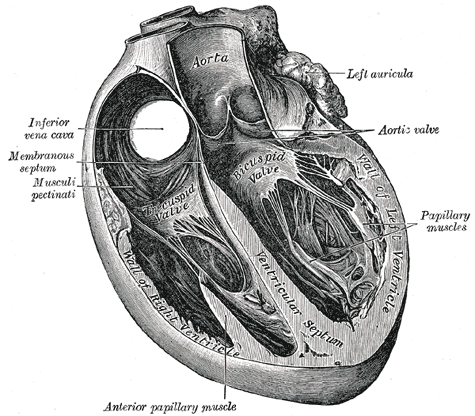
\includegraphics[width=0.7\textwidth]{figures/sample/Gray498.png} 
\caption[Four-chamber illustration of the human heart.]{Four-chamber illustration of the human heart.  Clockwise from upper-left: right atrium, left atrium, left ventricle, right ventricle.}
\label{fig:fourchamber}\end{figure}

The use of acoustic waves for medical diagnosis, inspired by naval sonar, was initially developed in the 1940s \cite{gagliardi_ultrasonography_1996}.  By 1954, the first clinically useful cardiac ultrasound -- examining motion of the mitral valve in stenosis -- was reported \cite{edler_ultrasonic_1957}.  These early scans were one-dimensional images (`A-mode'), sometimes repeated to generate a time axis (`M-mode').   The sector-scanning probe was developed in the 1970s \cite{bom_ultrasonic_1971,griffith_sector_1974}, leading to the `B-mode' that a modern cardiologist would recognise as an echocardiogram.



%% APPENDICES %% 
% Starts lettered appendices, adds a heading in table of contents, and adds a
%    page that just says "Appendices" to signal the end of your main text.
% \startappendices
% Add or remove any appendices you'd like here:
\chapter{\label{ch:appendix}Appendices}



%%%%% REFERENCES

% JEM: Quote for the top of references (just like a chapter quote if you're using them).  Comment to skip.
% \begin{savequote}[8cm]
% The first kind of intellectual and artistic personality belongs to the hedgehogs, the second to the foxes \dots
%   \qauthor{--- Sir Isaiah Berlin \cite{berlin_hedgehog_2013}}
% \end{savequote}

\setlength{\baselineskip}{0pt} % JEM: Single-space References

{\renewcommand*\MakeUppercase[1]{#1}%
\printbibliography[heading=bibintoc,title={\bibtitle}]}


\end{document}
